% !TEX program = pdflatex
\documentclass{article}
% FONTS
\usepackage[T1]{fontenc}
\usepackage{tgtermes}
\usepackage{amsmath}

% GEOMETRY
\usepackage[
  paper  = letterpaper,
  left   = 1.65in,
  right  = 1.65in,
  top    = 1.0in,
  bottom = 1.0in,
  ]{geometry}

% COLOR
\usepackage[usenames,dvipsnames]{xcolor}
\definecolor{shadecolor}{gray}{0.9}

% SPACING and TEXT
\usepackage[final,expansion=alltext]{microtype}
\usepackage[english]{babel}
\usepackage[parfill]{parskip}
\usepackage{afterpage}
\usepackage{framed}
\usepackage{nicefrac}

% COUNTERS
\renewcommand{\labelenumi}{\color{black!67}{\arabic{enumi}.}}
\renewcommand{\labelenumii}{{\color{black!67}(\alph{enumii})}}
\renewcommand{\labelitemi}{{\color{black!67}\textbullet}}

% FIGURES
\usepackage{graphicx}
\usepackage[labelfont=bf]{caption}
\usepackage[format=hang]{subcaption}

% TABLES
\usepackage{booktabs}

% BIBLIOGRAPHY
\usepackage{natbib}

% ALGORITHMS
\usepackage[algoruled]{algorithm2e}
\usepackage{listings}
\usepackage{fancyvrb}
\fvset{fontsize=\normalsize}

% HYPERREF
\usepackage[colorlinks,linktoc=all]{hyperref}
\usepackage[all]{hypcap}
\hypersetup{citecolor=Violet}
\hypersetup{linkcolor=black}
\hypersetup{urlcolor=MidnightBlue}

% CLEVEREF must come after HYPERREF
\usepackage[nameinlink]{cleveref}

% COLOR DEFINITIONS
\newcommand{\red}[1]{\textcolor{BrickRed}{#1}}
\newcommand{\orange}[1]{\textcolor{BurntOrange}{#1}}
\newcommand{\green}[1]{\textcolor{OliveGreen}{#1}}
\newcommand{\blue}[1]{\textcolor{MidnightBlue}{#1}}
\newcommand{\gray}[1]{\textcolor{black!60}{#1}}

% LISTINGS
\usepackage{listings}


% !TEX root = template.tex

% \DeclareRobustCommand{\mb}[1]{\ensuremath{\boldsymbol{\mathbf{#1}}}}
\DeclareRobustCommand{\mb}[1]{\mathbold{#1}}

% \newcommand{\KL}[2]{\ensuremath{\textrm{KL}\PARENS{#1\;\|\;#2}}}
\DeclareRobustCommand{\KL}[2]{\ensuremath{\textrm{KL}\left(#1\;\|\;#2\right)}}

\DeclareMathOperator*{\argmax}{arg\,max}
\DeclareMathOperator*{\argmin}{arg\,min}

\renewcommand{\mid}{~\vert~}
\newcommand{\g}{\mid}
\newcommand{\prm}{~;~}

\newcommand{\mba}{\mb{a}}
\newcommand{\mbb}{\mb{b}}
\newcommand{\mbc}{\mb{c}}
\newcommand{\mbd}{\mb{d}}
\newcommand{\mbe}{\mb{e}}
\newcommand{\mbg}{\mb{g}}
\newcommand{\mbh}{\mb{h}}
\newcommand{\mbi}{\mb{i}}
\newcommand{\mbj}{\mb{j}}
\newcommand{\mbk}{\mb{k}}
\newcommand{\mbl}{\mb{l}}
\newcommand{\mbm}{\mb{m}}
\newcommand{\mbn}{\mb{n}}
\newcommand{\mbo}{\mb{o}}
\newcommand{\mbp}{\mb{p}}
\newcommand{\mbq}{\mb{q}}
\newcommand{\mbr}{\mb{r}}
\newcommand{\mbs}{\mb{s}}
\newcommand{\mbt}{\mb{t}}
\newcommand{\mbu}{\mb{u}}
\newcommand{\mbv}{\mb{v}}
\newcommand{\mbw}{\mb{w}}
\newcommand{\mbx}{\mb{x}}
\newcommand{\mby}{\mb{y}}
\newcommand{\mbz}{\mb{z}}

\newcommand{\mbA}{\mb{A}}
\newcommand{\mbB}{\mb{B}}
\newcommand{\mbC}{\mb{C}}
\newcommand{\mbD}{\mb{D}}
\newcommand{\mbE}{\mb{E}}
\newcommand{\mbF}{\mb{F}}
\newcommand{\mbG}{\mb{G}}
\newcommand{\mbH}{\mb{H}}
\newcommand{\mbI}{\mb{I}}
\newcommand{\mbJ}{\mb{J}}
\newcommand{\mbK}{\mb{K}}
\newcommand{\mbL}{\mb{L}}
\newcommand{\mbM}{\mb{M}}
\newcommand{\mbN}{\mb{N}}
\newcommand{\mbO}{\mb{O}}
\newcommand{\mbP}{\mb{P}}
\newcommand{\mbQ}{\mb{Q}}
\newcommand{\mbR}{\mb{R}}
\newcommand{\mbS}{\mb{S}}
\newcommand{\mbT}{\mb{T}}
\newcommand{\mbU}{\mb{U}}
\newcommand{\mbV}{\mb{V}}
\newcommand{\mbW}{\mb{W}}
\newcommand{\mbX}{\mb{X}}
\newcommand{\mbY}{\mb{Y}}
\newcommand{\mbZ}{\mb{Z}}

\newcommand{\mbalpha}{\mb{\alpha}}
\newcommand{\mbbeta}{\mb{\beta}}
\newcommand{\mbdelta}{\mb{\delta}}
\newcommand{\mbepsilon}{\mb{\epsilon}}
\newcommand{\mbchi}{\mb{\chi}}
\newcommand{\mbeta}{\mb{\eta}}
\newcommand{\mbgamma}{\mb{\gamma}}
\newcommand{\mbiota}{\mb{\iota}}
\newcommand{\mbkappa}{\mb{\kappa}}
\newcommand{\mblambda}{\mb{\lambda}}
\newcommand{\mbmu}{\mb{\mu}}
\newcommand{\mbnu}{\mb{\nu}}
\newcommand{\mbomega}{\mb{\omega}}
\newcommand{\mbphi}{\mb{\phi}}
\newcommand{\mbpi}{\mb{\pi}}
\newcommand{\mbpsi}{\mb{\psi}}
\newcommand{\mbrho}{\mb{\rho}}
\newcommand{\mbsigma}{\mb{\sigma}}
\newcommand{\mbtau}{\mb{\tau}}
\newcommand{\mbtheta}{\mb{\theta}}
\newcommand{\mbupsilon}{\mb{\upsilon}}
\newcommand{\mbvarepsilon}{\mb{\varepsilon}}
\newcommand{\mbvarphi}{\mb{\varphi}}
\newcommand{\mbvartheta}{\mb{\vartheta}}
\newcommand{\mbvarrho}{\mb{\varrho}}
\newcommand{\mbxi}{\mb{\xi}}
\newcommand{\mbzeta}{\mb{\zeta}}

\newcommand{\mbDelta}{\mb{\Delta}}
\newcommand{\mbGamma}{\mb{\Gamma}}
\newcommand{\mbLambda}{\mb{\Lambda}}
\newcommand{\mbOmega}{\mb{\Omega}}
\newcommand{\mbPhi}{\mb{\Phi}}
\newcommand{\mbPi}{\mb{\Pi}}
\newcommand{\mbPsi}{\mb{\Psi}}
\newcommand{\mbSigma}{\mb{\Sigma}}
\newcommand{\mbTheta}{\mb{\Theta}}
\newcommand{\mbUpsilon}{\mb{\Upsilon}}
\newcommand{\mbXi}{\mb{\Xi}}

\newcommand{\mbone}{\mbf{1}}
\newcommand{\mbzero}{\mbf{0}}


\newcommand{\dif}{\mathop{}\!\mathrm{d}}
\newcommand{\diag}{\textrm{diag}}
\newcommand{\supp}{\textrm{supp}}

\newcommand{\E}{\mathbb{E}}
\newcommand{\Var}{\mathbb{V}\textrm{ar}}
\newcommand{\bbH}{\mathbb{H}}

\newcommand{\bbN}{\mathbb{N}}
\newcommand{\bbZ}{\mathbb{Z}}
\newcommand{\bbR}{\mathbb{R}}
\newcommand{\bbS}{\mathbb{S}}

\newcommand{\cA}{\mathcal{A}}
\newcommand{\cB}{\mathcal{B}}
\newcommand{\cC}{\mathcal{C}}
\newcommand{\cD}{\mathcal{D}}
\newcommand{\cE}{\mathcal{E}}
\newcommand{\cF}{\mathcal{F}}
\newcommand{\cG}{\mathcal{G}}
\newcommand{\cH}{\mathcal{H}}
\newcommand{\cI}{\mathcal{I}}
\newcommand{\cJ}{\mathcal{J}}
\newcommand{\cK}{\mathcal{K}}
\newcommand{\cL}{\mathcal{L}}
\newcommand{\cM}{\mathcal{M}}
\newcommand{\cN}{\mathcal{N}}
\newcommand{\cO}{\mathcal{O}}
\newcommand{\cP}{\mathcal{P}}
\newcommand{\cQ}{\mathcal{Q}}
\newcommand{\cR}{\mathcal{R}}
\newcommand{\cS}{\mathcal{S}}
\newcommand{\cT}{\mathcal{T}}
\newcommand{\cU}{\mathcal{U}}
\newcommand{\cV}{\mathcal{V}}
\newcommand{\cW}{\mathcal{W}}
\newcommand{\cX}{\mathcal{X}}
\newcommand{\cY}{\mathcal{Y}}
\newcommand{\cZ}{\mathcal{Z}}

\newcommand{\Gam}{\textrm{Gam}}
\newcommand{\InvGam}{\textrm{InvGam}}

\usepackage{amsfonts} 
\begin{document}

\title{Effect of prescribed fire on the wildfire in California}
\date{\today}
\author{Shuonan Chen, sc4417}

\maketitle

\begin{abstract}
While wildfire in California is being a big thread as a part of the product of the climate change, not much is known about their impact. Current analysis on wildfire oftentimes assume that the consequences caused by wildfire is uniform across the regions. Here we take a deeper analysis by building a model based on Gaussian Process and explore if previously prescribed fire and hydrologic regions have impact on the severity of wildfire in given regions. We found that the prescribed fire has minor impact on the wildfire severity but the hydrologic region has a large effect. The model can be further expanded to incorporate more explanatory variables which will help the climate scientists to study the best strategy to minimize the negative effect of wildfire. 
\end{abstract}



\section{Introduction}
California wildfire are mainly caused by either natural events such as lightning and human activities. 
Even though from the environmental perspective, wildfire promotes the revegetation and is a part of natural proces, they also have many negative impact both socioecologically and environmentally. For instance, they destroy the habitat for animals and plants, disrupt the power and water supply and transportation, and also can worsen the air pollution \cite{moritz2014learning}. 
With climate change, the California's rainy winter season is getting shorter and in the recent years we have witnessed an increase on the wildfire cases and the negative impact caused, accompanied with the extreme heat and driness in the area. 
While ecologically it is almost impossible to completely prevent the wildfire from happening, the severity of the events can vary when it happens due to different factors, such as the vegetation conditions, topology, water contents in the soil, and previously burned history. 



To reduce the disruptive effects of wildfire, an age-old practise is induce the planned fire by human-beings, namely ``prescribed burn''. Prescribed burn has been used for a long time for the forest management, mainly with the aim to get rid of the small trees, to further reduce the fuel load for the wildfires. It has been increasingly acknowledged that prescribed fires are being useful to maintain the forest. 


Severity of the wildfire is hard to estimate, and even if we can estimate the severity, the challenge remains to understand the relationship between the wildfire and the other factors, which makes it difficult to gain insights on practical study. For instance, an effort was made to estimate the Giant Sequoia mortality rate in the wildfire \cite{stephenson2021preliminary}. However in this study, the authors made a simplified assumption that the mortality of Giant Sequoia is proportional to the reported severity of the wildfire. This might be the case if we do not consider the other factors such as landscape and vegetation. However the assumption will be problematic if, for example, some parts of the grove are burned more servery if the landscape is tilted, or the soil water contents are significantly different from the other regions with the similar wildfire severity. 


Developing a method to explore the relationships of wildfire and the other factors listed above would be helpful. Notably, in the previous work \cite{stephenson2021preliminary}, in order to estimate the Giant Sequoia grove mortality rate associated with 2020 Castle fire, the authors made an assumption that the mortality rate is proportional to the severity of the wildfire. This admittedly is a reasonable assumption given that there is no information to deny this assumption. However, more detailed understanding of what factors might be relevant to the wildfire will benefit for both the analysis and the future wildfire prevention. 

Here we used the limited available data source to understand these impact on wildfire severity. Particularly, we wanted to see how much the prescribed fire burn has impact on the burn severity of wildfires. Through this work, we provide the possible modeling approach to understand what factors might have the impact to the California wildfire severities, and used this modeling framework to understand the effects of hydrolic region and the prescribed fire at the same region. This work can be extended to give a more systematic understanding. In particular, the framework can be used to provide insights into the analytical assumptions made by \cite{stephenson2021preliminary}, and give a more accurate estimate of the mortality rate of Giant Sequoia. 


\section{Methods}
\subsection*{Data source}
The main source of the data used was three folds. The first is the burned area by wildfire, obtained from Rapid Assessment of Vegetation Condition After Wildfire (RAVG).


The second data source is the hydrologic region, which was obtained from California Department of Forestry and Fire Protection's Fire and Resource Assessment Program (FRAP) (under name \textit{CALWATER 2.2.1}). 10 hydrologic region data was used. The reason of choosing this dataset was for several reasons. First, this is the most accessible data to reflect different regions in California. Topgraphical data was not found under limited time for this analysis. Second, it captures both the water contents as well as the other geographical characteristics in California. 

The third data source is the prescribed fire, it is obtained from Geographic information sytems (GIS) service (under name \textit{Prescribed Fire Burns - California [ds397]}, version from October 2022). As for RAVG data, only the data from the year 

\subsection*{Data preprocessing}
First of all, for wildfire burned area from RAVG and the prescribed fire area, it is not clear how to extract the exact locations of the regions. Therefore, we simplified the data by taking the 2D coordinates mass center of each region. In order to reduce the size of the data, we took a grid of size 20km as a preprocessing step; this is also helpful to ensure that multiple covariates exist in the same region (20km by 20km grid). In the future when more data is available this can be loosen to increase the number of datapoints. 

For the burned area, since the data had a highly skewed distribution, log-transformation was done before modeling. The original unit for these were ``Acres''. 
The hydrologic regions are the categorical data and therefore the features are converted to 10 binary values. The other explanatory variable, prescribed fire region, is normalized between 0 and 1.





\subsection*{Data Notations}
Here we introduce the notations used throughout in this report. We use $i$ to denote the datapoint, and $x_i \in \mathbb{R}^2$ is the location on the 2D grid space, for datapoints $i = 1,....N$. Meanwhile, we will incorporate the other explanatory variables as $z_i \in \mathbb{R}^P$, where $p$-th covariates are the $p$-th explanatory variable. In this paper, $P=11$, but it is easily extended with data with more explanatory variables. 

% The covariates include the vegetation, prescribed fire area, and humidity at location $x_i$, but can be expanded further. 



\subsection*{Model}
The model is described as follows. 
\begin{align*}
    y_i &\sim \text{normal}(\mu_i, \eta),\\
    \mu_i &= f_1(x_i) + f_2(z_i),\\
    f_1(x) &\sim GP(0,k(x,x')),\\
    f_2(z) &= z\cdot \beta.
\end{align*}


\subsection*{Implementation}
The model was written in a programming language Stan \cite{carpenter2017stan,riutort2020practical}, and was executed using CmdStan interface from python (Cmdstanpy version 1.0.8). Stan uses HMC methods particularly Non-U-turn Sampler (NUTS). There are many libraries available to run GP, but Stan turns out to give the most flexibility in terms of writing out the model, and provides the possibility to further extend the model to include additional explanatory variables which is critical for the future study. 

The kernel function was implemented with the exponentiated quadratic kernel, through \texttt{cov\_exp\_quad}.



\section{Results}
The 

\begin{figure*}[t!]
  \centering
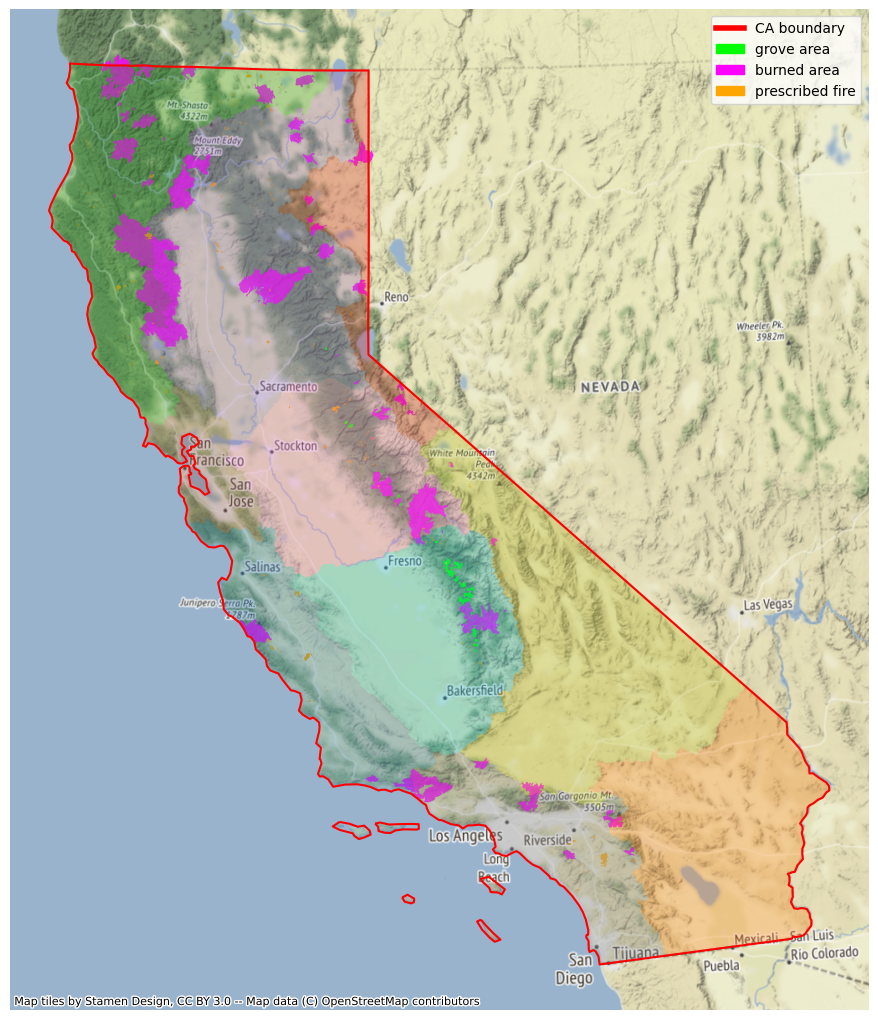
\includegraphics[width=0.45\textwidth]{latex_template/figs/prescribed_0.png}
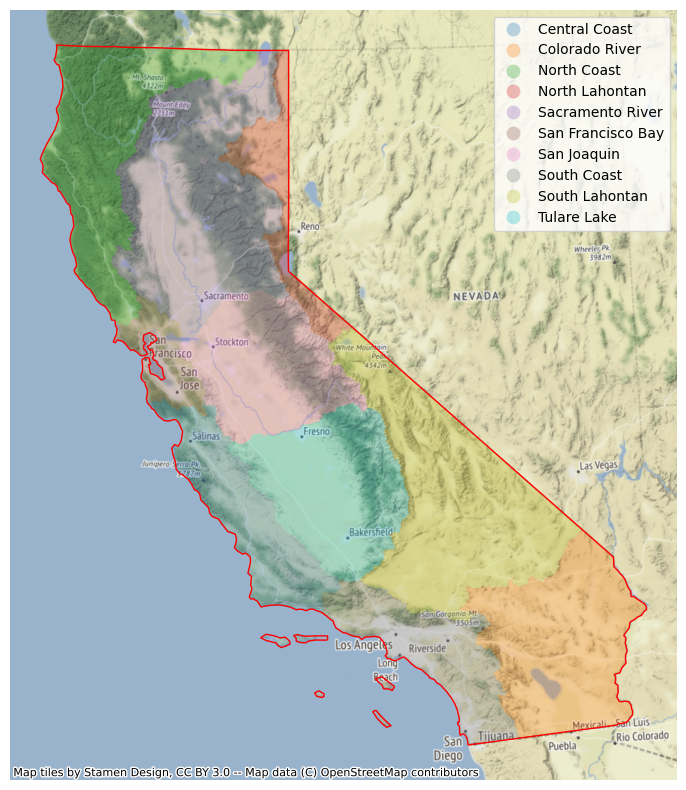
\includegraphics[width=0.45\textwidth]{figs/HRarea_1.png}

\caption{\textbf{Data description.} Left panel shows the prescribed fire (orange) location and area, as well as the burned area by wildfire (magenta) along with their locations. Right panel shows the hydrogen regions features in California where each color represents one category. }
\label{fig:data}
\end{figure*}


\begin{figure*}[!h]
  \centering
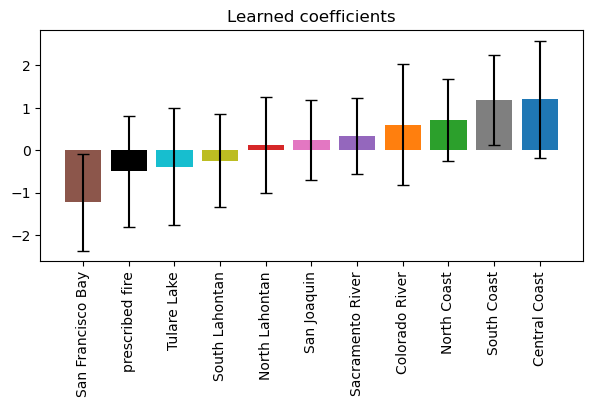
\includegraphics[width=0.5\textwidth]{latex_template/figs/betas.png}
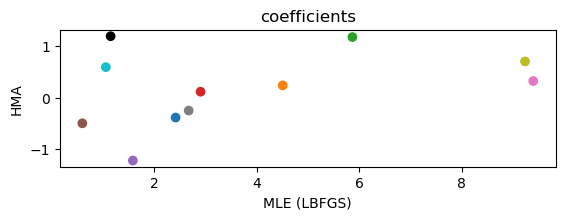
\includegraphics[width=0.5\textwidth]{latex_template/figs/hmc_mle.png}
\caption{\textbf{Parameter estimation results.} Left plot is the estimated mean of the coefficients ($\beta$ ) for all 11 explanatory variables listed. The errorbars represents the standard deviation of MCMC samplings. The right panel is the comparison of estimated coefficients between MLE using Stan's \texttt{optimization} algorithm (x-axis) versus those estimated using MCMC (y-axis). }
\label{fig:data}
\end{figure*}








\begin{figure*}[!t]
  \centering
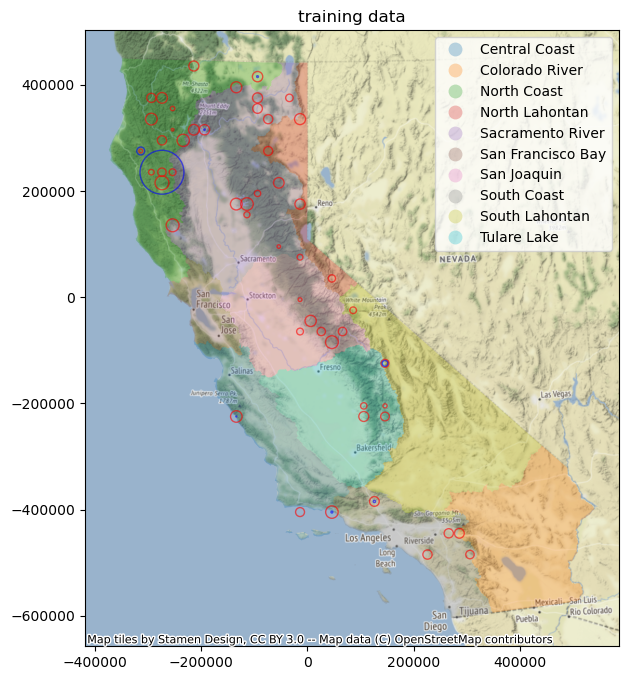
\includegraphics[width=0.45\textwidth]{latex_template/figs/trained_rez.png}
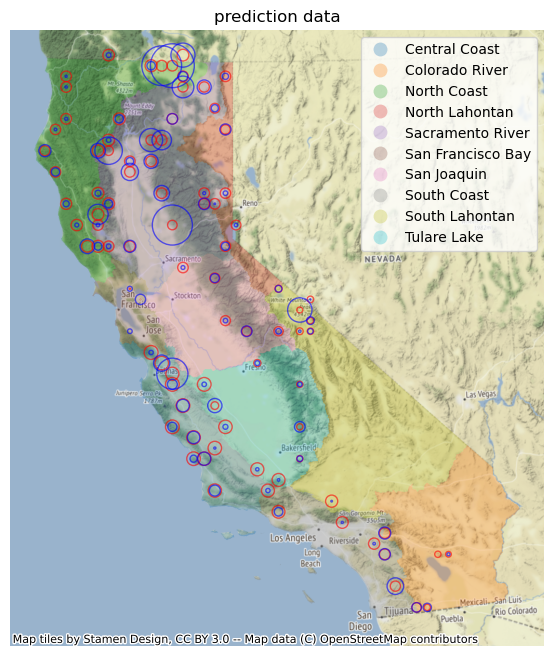
\includegraphics[width=0.45\textwidth]{latex_template/figs/predicted_rez.png}
\caption{\textbf{Relationships between the burned area from wildfire and the prescribed fire. } Left panel shows all the explanatory variables overlaid with the wildfire burned area and the geographical locations in California. Right panel shows all the explanatory variables overlaid with the the geographical locations in California, as well as \textit{predicted} wildfire burned area. Prescribed fire are shown in blue circles and ground-truth or predicted burned area are shown in red circles. }
\label{fig:data}
\end{figure*}





\section{Discussion}
2D Gaussian Process in the field of geostatistical is essentially the ``kringing'' problem. Using the flexibility of MCMC sampling in Stan, we extended the simple 2D GP to incorporate the explanatory variables which do not necessarily needed to be modeled as the GP inputs. This gives much more flexibility in modeling and allows us to be more expressive on what factors should be considered. 


The discrepancy on the point estimation and the HMC (NUTS) estimation is concerning. This might be the suboptimal model specification. It is possible that point estimation found the local minima whereas the samplign approach found the global optimam. It is also possible there is some parameter identifiability issues here, which needs to be investigated further. 

Many covariates are not included due to the limtied data that could be found. This includes topographical data that captures the landscapes more accurately, as well as the vegetation conditions. More importantly, in order to assess the relationships 



\clearpage
\bibliographystyle{unsrt}

\bibliography{ref}


\end{document}
